\documentclass[12pt]{article}
\usepackage[utf8]{inputenc}
\usepackage[T1]{fontenc}
\usepackage{amsmath,amssymb,amscd,tikz}
\usepackage{geometry}
\geometry{margin=2.5cm}

\begin{document}

\section*{Curs 3 -- Pagina 5}

\noindent $(M_2(\mathbb{R}),\cdot)$ -- monoid.

\noindent $H\subseteq G$, $G$ = grup.

\begin{enumerate}
\item[1)] $(\forall)\, x,y\in H \Rightarrow xy\in H$
\item[2)] $(\forall)\, x\in H \Rightarrow x^{-1}\in H$
\end{enumerate}
\hspace{1cm}$\Bigg\} \Rightarrow (H,\cdot) = $ grup.

\noindent $x\in H \Rightarrow x^{-1}\in H \Rightarrow e\in H$.

\bigskip
\noindent\underline{\textbf{Dem.}} -- evidentă.

\bigskip
\noindent (Legea de compoziție indusă pe o mulțime cât\footnote{cuvântul exact e neclar în original -- ar putea fi ,,factor'' în loc de ,,cât''.}.)

\[
(S,\varphi,R), \qquad S\neq\varnothing
\]
\noindent $\varphi$ = lege de compoziție pe $S$.\\
$R$ = relație de echivalență pe $S$.

\[
\begin{CD}
S\times S @>\varphi>> S\\
@V{p\times p}VV @VV{p}V\\
S/R\times S/R @>\varphi^*>> S/R
\end{CD}
\]
\noindent $p(a) = \hat a$.\footnote{simbolul exact folosit în original pentru proiecția canonică e neclar -- am ales $p$.}

\noindent $(p\times p)(a,b) = (\hat a,\hat b)$.

\noindent $\varphi^*(\hat a,\hat b) \overset{\text{def}}{=} \varphi(a,b)$

\noindent din teorema de factorizare $\Rightarrow \exists\, \varphi^* \Rightarrow$ e unică.

\begin{center}
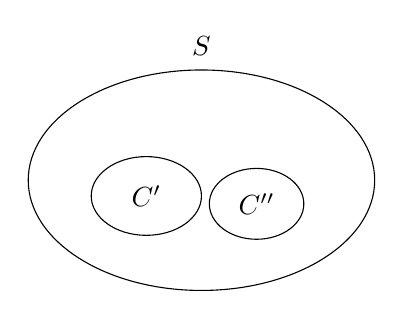
\begin{tikzpicture}
\draw (0,0) ellipse (2.2 and 1.4);
\node at (0,1.7) {$S$};
\draw (-0.7,-0.2) ellipse (0.7 and 0.5);
\draw (0.7,-0.3) ellipse (0.6 and 0.45);
\node at (-0.7,-0.2) {$C'$};
\node at (0.7,-0.3) {$C''$};
\end{tikzpicture}
\end{center}

\noindent $a\in C',\ b\in C'' \Rightarrow \hat a = C',\ \hat b = C''$. \quad $\varphi^*(\hat a,\hat b) = \varphi(a,b)$

\noindent Fie $a'\in C'$ şi $b'\in C''$ $\Rightarrow$ $\varphi^*(\hat a',\hat b') = \varphi(a',b')$

\bigskip
\noindent\underline{\textbf{Def:}} Fie $S\neq\varnothing$, $(S,\cdot)$. O relație de echivalență $R$ pe $S$ s.n. \textbf{congruență} pe $S$ dacă

\noindent din $aRa'$ şi $bRb' \Rightarrow abRa'b'$

\noindent (sau $a\sim a'$ şi $b\sim b'$) $\Rightarrow$ $(ab\sim a'b')$.

\bigskip
\noindent\underline{\textbf{Exp:}} $(\mathbb{Z},+,\cdot)$ \qquad $n \mid x-y$

\noindent $(\mathbb{Z}_n,+,\cdot)$.

\noindent $a\equiv a' \pmod n$ şi $b\equiv b' \pmod n$ $\Rightarrow$ $ab\equiv a'b' \pmod n$,

\noindent $(a+b\equiv a'+b' \pmod n)$.

\[
a-a' = un,\qquad b-b'=tn
\]
\[
a+b-(a'+b') = un+tn = (u+t)n
\]
\[
ab = (a'+un)(b'+tn) = a'b' + n(\,ub'+a't+unt\,)
\]
\noindent\textit{(acest ultim bloc de calcul e reconstituit după cifre foarte mici/înghesuite în original -- te rog verifică variabilele $u,t$ şi expresia finală.)}

\end{document}
